\documentclass[fontsize=11pt]{article}
\usepackage{lmodern}
\usepackage[protrusion=true,expansion=true]{microtype}
\usepackage[svgnames]{xcolor}  % Colours by their 'svgnames'
\usepackage[margin=0.75in]{geometry}
\textheight=700px
\usepackage{url}
\usepackage{lmodern} % Allow arbitrary font sizes
\usepackage{textcomp}

\usepackage{amssymb}
\usepackage{fontawesome5}
\usepackage{hyperref}
\hypersetup{
    colorlinks=false,
    pdfborder={0 0 0},
}

\usepackage{graphicx}

\usepackage[utf8]{inputenc}
\usepackage[T2A]{fontenc}
\usepackage[english,russian]{babel}

%% Define a new 'modern' style for the url package that will use a smaller font.
\makeatletter
\def\url@modernstyle{
  \@ifundefined{selectfont}{\def\UrlFont{\sf}}{\def\UrlFont{}}}
\makeatother
\urlstyle{modern} %% And use the newly defined style.

\frenchspacing              % Better looking spacings after periods
\pagestyle{empty}           % No pagenumbers/headers/footers

\renewcommand{\familydefault}{\sfdefault}

%%% Custom sectioning (sectsty package)
%%% ------------------------------------------------------------
\usepackage{sectsty}

\sectionfont{                 % Change font of \section command
  \sectionrule{0pt}{0pt}{-5pt}{3pt}}

%%% Macros
%%% ------------------------------------------------------------
\newlength{\spacebox}
\settowidth{\spacebox}{8888888888}      % Box to align text
\newcommand{\sepspace}{\vspace*{1em}}   % Vertical space macro

\newcommand{\MyName}[1]{ % Name
    \Huge \centering #1
    \par \normalsize \normalfont}

\newcommand{\NewPart}[1]{\section*{#1}}

\newcommand{\PersonalEntry}[2]{
    \noindent\hangindent=2em\hangafter=0 % Indentation
    \parbox{\spacebox}{                  % Box to align text
    \textit{#1}}                      % Entry name (birth, address, etc.)
    \hspace{1.5em} #2 \par}              % Entry value

\newcommand{\SkillsEntry}[2]{                % Same as \PersonalEntry
    \noindent\hangindent=2em\hangafter=0 % Indentation
    \parbox{\spacebox}{                  % Box to align text
    \textit{#1}}                    % Entry name (birth, address, etc.)
    \hspace{1.5em} #2 \par}              % Entry value

\newcommand{\AwardsEntry}[2]{                % Same as \PersonalEntry
    \noindent\hangindent=2em\hangafter=0 % Indentation
    \parbox{\spacebox}{                  % Box to align text
    \textit{#1}}                    % Entry name (birth, address, etc.)
    \hspace{1.5em} #2 \par}              % Entry value

\newcommand{\ProgrammingEntry}[2]{
    \noindent \textbf{#1} \hfill      % Study

    \noindent \small #2 % Description
    \normalsize \par}

\newcommand{\EducationEntry}[4]{
    \noindent \textbf{#1} \hfill      % Study
    \colorbox{Black}{
      \parbox{10em}{
      \color{White} \centering #2}} \par   % Duration
    \noindent \textit{#3} \par        % School
    \noindent\hangindent=2em\hangafter=0 \small #4 % Description
    \normalsize \par}

\newcommand{\WorkEntry}[3]{       % Same as \EducationEntry
    \noindent \large \textbf{#1} \hfill      % Jobname
    \colorbox{Black}{%
      \parbox{10em}{%
      \color{White} \centering #2}} \par  % Duration
    \noindent \small #3 % Description
    \normalsize \par}

\newcommand{\ProjectEntry}[4]{         % Similar to \EducationEntry
    \noindent \textbf{#1} \noindent \textit{#3} \hfill {#2} \par
    \noindent \small #4 % Description
    \normalsize \par}

\newcommand{\AwardEntry}[4]{         % Similar to \EducationEntry
    \noindent \textbf{#1} \noindent \textit{#3} \hfill {#2} \par
    \noindent \small #4 % Description
    \normalsize \par}
    \begin{document}



\begin{minipage}{0.2\textwidth}% adapt widths of minipages to your needs
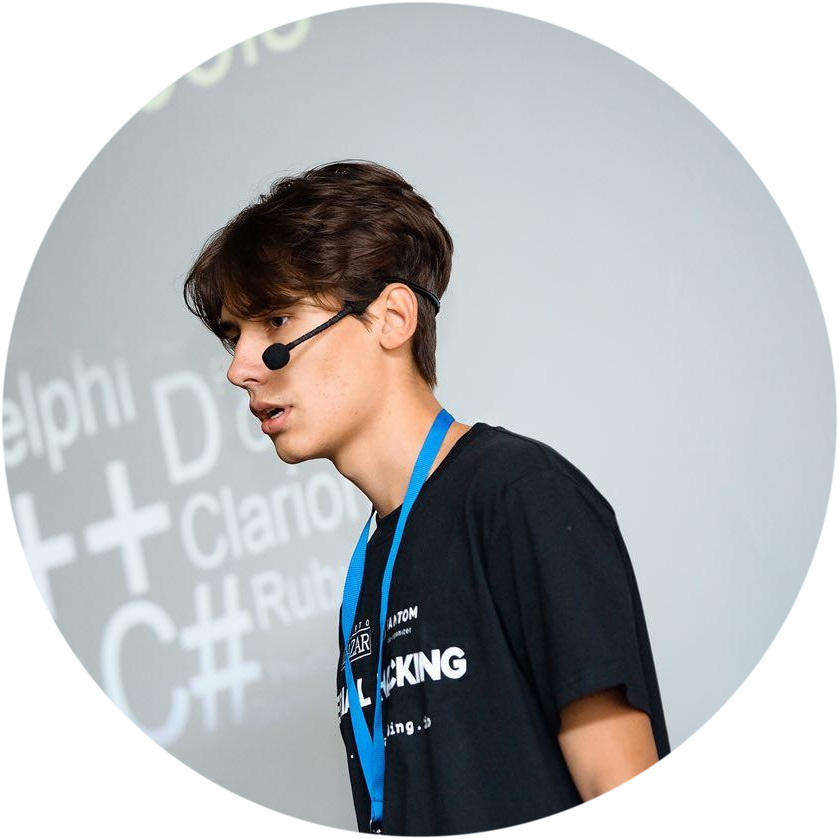
\includegraphics[width=4cm]{me.png}
\end{minipage}%
\hfill%
\begin{minipage}{14cm}\raggedright
\bigskip
\bigskip
\bigskip
\bigskip
\bigskip
\bigskip
\MyName{Дмитрий Инютин}
\bigskip
{inyutin.da@gmail.com | 89154336070 | \href{https://t.me/inyutin}{\faTelegram \, Telegram} | \href{https://github.com/inyutin}{\faGithub \, Github} | Москва}
\end{minipage}


%%% Work experience
%%% ------------------------------------------------------------ц

%%%
%%% Education
%%% ------------------------------------------------------------
\NewPart{Образование}{}
\EducationEntry
{Бакалавр в области прикладной математики и информатики}
{2016 - 2020}
{Московский физико-технический институт, ФИВТ ПМИ.}

\NewPart{Опыт работы}{}
\WorkEntry
{Ассистент в МФТИ}
{Весна 2019}
{Помогаю на курсе "Теории и практики многопоточной синхронизации". \\ Проверяю домашние задания у студентов и стараюсь объяснять непонятое на семинаре и лекции.}

\bigskip

\WorkEntry
{Интерн в Jetbrains}
{Лето 2018}
{Работал над новым продуктом компании - веб-средой для анализа данных. \\ Я сделал онлайн редактор кода более дружелюбным и удобным при взаимодействии с мобильных устройств.}

%%% Skills
%%% ------------------------------------------------------------
\NewPart{Знание языков программирования}{}
\ProgrammingEntry
{C++ \bigstar \bigstar \bigstar}
{Активно использую для учебных проектов. \\ Хорошо знаком со стандартными контейнерами и примитивами синхронизации.}
\bigskip
\ProgrammingEntry
{Python \bigstar \bigstar \bigstar}
{Постоянно использую для написания небольших программ, скриптов.}
\bigskip
\ProgrammingEntry
{Java \bigstar \bigstar}
{Работал с Java GWT и писал небольшой backend на Spring Framework. \\
Также написал несколько небольших Android-приложений.}
\bigskip
\ProgrammingEntry
{JavaScript \bigstar \bigstar}
{Написал небольшой сервер для для блокчейн-приложения на NodeJs.}
\bigskip
\ProgrammingEntry
{Go \bigstar}
{Реализовал игрушечную версию CASPaxos - Replicated State Machine without logs.}

\NewPart{Дополнительные навыки}{}
\SkillsEntry{Блокчейн}{Работал с api Ethereum (web3js), писал приложения, использующую эту технологию.}
\SkillsEntry{Инструменты}{Git, Linux}

%%% Awards
%%% ------------------------------------------------------------
\NewPart{Участие в хакатонах}{}

\AwardEntry{Cryptobazar, }{Победитель}
{Москва, Сентябрь - Декабрь 2018}
{Различные приложения так или иначе связанные с блокчейном: парное шифрование, \\ мобильный криптокошелёк, виртуальная машина для языка WebAssembly.}
\sepspace
\AwardEntry{Phystech.Genesis,}{Победитель}
{Москва, Сентябрь 2018}
{Андроид приложение для туристов, которое находит интересные маршруты.}
\sepspace
\AwardEntry{Global Changers 2,}{Победитель}
{Москва, Март 2018}
{Вебсервис, который создает интерактивные Customer Journey Map.}
\sepspace
\AwardEntry{Birth.Hack,}{Участник}
{Moscow, April 2018}
{Вебсайт, где пользователи могут смотреть спортивные матчи вместе, используя видеочат.}
\sepspace
\AwardEntry{Global Changers 1,}{Победитель}
{МФТИ, Март 2018}
{Видеоплатформа, которая поощряет пользователей за их социальную активность (загрузку видео и комментарии).}
\sepspace
\AwardEntry{mABBYYlity,}{Участник}
{МФТИ, Октябрь 2017}
{Небольшой телеграмм-бот, который по фотографии штрихкода товара показывает отзывы покупателей \\ и цены в близжайших магазинах.}

\NewPart{Проекты}{}
\ProgrammingEntry
{ViBoard}
{Проект, выросший из хакатона Global Changers 1. Это был видеосервис, где все данные хранились распределенно в сети IPFS. Мы пытались построить экономику, основанную на комьюнити. Каждый день появлялось некоторое число новых монеток, которые раздавались самым "залайканым" \space пользователям за день. Подразумевалось, их стоимость будет обеспечена популярность платформы, но проект так и не взлетел.}
\bigskip
\ProgrammingEntry
{CASPaxos}
{CASPaxos - это распределенный регистр без лога. \\ Главная идея CASPaxos это попытка реплицировать состояние регистра, а не лог. Я хотел разобраться как он устроен и написал свою небольшую реализацию.}
\bigskip
\ProgrammingEntry
{MakeGood}
{Совсем маленький скрипт на питоне, который поднимает настроение, показывая позитивную и смешную картинку.}

\end{document}
